\documentclass[a4paper,12pt]{article}
\usepackage{amsmath} \usepackage{amsthm}
\usepackage[croatian]{babel}
\usepackage{graphicx}
\usepackage{amssymb} \usepackage{fancybox}
\usepackage{latexsym} 
\usepackage{enumerate}
\usepackage{subfigure}
\addtolength{\hoffset}{-1cm} \addtolength{\textwidth}{2cm}
\addtolength{\topmargin}{-2.5cm} \addtolength{\textheight}{3cm}

\newtheoremstyle{zad}% name
  {0.3cm}%      Space above
  {10pt}%      Space below
  {}%         Body font
  {}%         Indent amount (empty = no indent, \parindent = para indent)
  {\bf}% Thm head font
  {.}%        Punctuation after thm head
  {\newline}%     Space after thm head: " " = normal interword space;
        %       \newline = linebreak
  {}%         Thm head spec (can be left empty, meaning `normal')

\theoremstyle{zad}
\newtheorem{zadatak}{Zadatak}

\begin{document}
%\thispagestyle{empty}
\begin{center}
\shadowbox{\Large Modeliranje svijećnjaka}\\[2pt]
\end{center}
\noindent Modeliranje svije\'cnjaka prikazanog na slici \ref{slika1} objasnit \'cemo u nekoliko koraka. Pritom nam treba nekoliko matemati\v{c}kih formula.\par\vspace*{5pt}
\begin{figure}[!h]
\centering
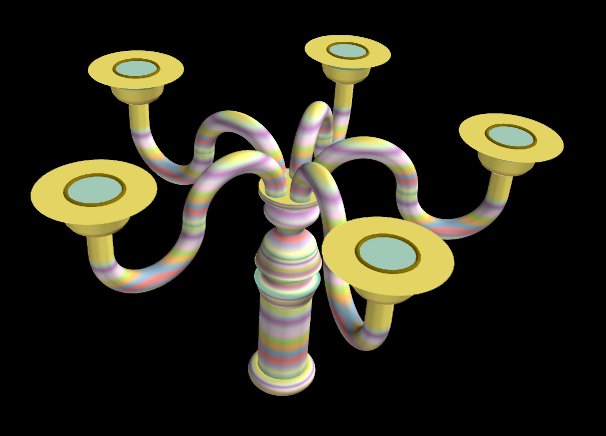
\includegraphics[scale=0.25]{slika1.png}
\vspace*{-10pt}
\caption{}
\label{slika1}
\end{figure}

\noindent Ako je u $yz$-ravnini zadana krivulja
$c:I\to\mathbb{R}$ parametarskim jednad\v{z}bama $$c(u)=\big(0,g(u),h(u)\big),$$
tada parametarske jednad\v{z}be plohe dobivene rotacijom te krivulje oko $z$-osi glase
\begin{align*}
x&=g(u)\sin{v}\\
y&=g(u)\cos{v}\\
z&=h(u)
\end{align*}
pri \v{c}emu je $u\in I,\ v\in[0,2\pi]$. Nadalje, rotacija $R_{z,\phi}$ oko $z$-osi za kut $\phi$ ima matri\v{c}ni prikaz
$$R_{z,\phi}=\begin{bmatrix}\cos{\phi}&-\sin{\phi}&0\\ \sin{\phi}&\cos{\phi}&0\\ 0&0&1\end{bmatrix}.$$
Dakle, rotacija oko $z$-osi za kut $\phi$ preslikava to\v{c}ku $(x,y,z)$ u to\v{c}ku
$$\begin{bmatrix}\cos{\phi}&-\sin{\phi}&0\\ \sin{\phi}&\cos{\phi}&0\\ 0&0&1\end{bmatrix}\begin{bmatrix}x\\ y\\ z\end{bmatrix}=
\begin{bmatrix}x\cos{\phi}-y\sin{\phi}\\ x\sin{\phi}+y\cos{\phi}\\ z\end{bmatrix}$$
odnosno
$$(x,y,z)\mapsto (x\cos{\phi}-y\sin{\phi},\,x\sin{\phi}+y\cos{\phi},\,z).$$
Parametarske jednad\v{z}be du\v{z}ine koja spaja to\v{c}ke $T_1(x_1,y_1,z_1)$ i $T_2(x_2,y_2,z_2)$ mo\v{z}emo zapisati u obliku
\begin{align*}
x&=x_1+(x_2-x_1)t\\
y&=y_1+(y_2-y_1)t,\quad t\in[0,1].\\
z&=z_1+(z_2-z_1)t
\end{align*}
Dio svije\'cnjaka prikazan na slici \ref{slika2} možemo modelirati pomo\'cu sljede\'ce dvije plohe koje su dijelovi torusa:
\begin{alignat*}{2}
x&=19+(13+3\cos{v_1})\cos{u_1}&\qquad\qquad x&=45+(13+3\cos{v_2})\cos{u_2}\\[3pt]
y&=3\sin{v_1}& y&=3\sin{v_2}\\[3pt]
z&=78+(13+3\cos{v_1})\sin{u_1}& z&=78+(13+3\cos{v_2})\sin{u_2}
\end{alignat*}
Pritom je $u_1\in[0,\pi],\,v_1\in[0,2\pi],\,u_2\in[\pi,2\pi],\,v_2\in[0,2\pi]$.\vspace*{5pt}
\begin{figure}[!h]
\centering
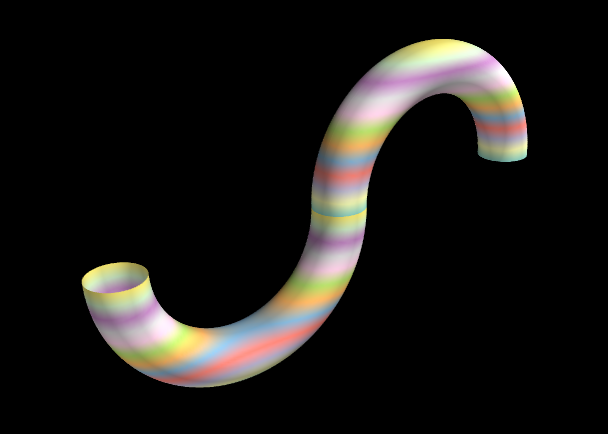
\includegraphics[scale=0.25]{slika2.png}
\vspace*{-10pt}
\caption{}
\label{slika2}
\end{figure}\vspace*{5pt}

\noindent Modeliranje oblika prikazanog na slici \ref{slika3a} opisat \'cemo u nekoliko koraka.\par\vspace*{5pt}
\begin{figure}[!h]
\centering
\subfigure[dio]{
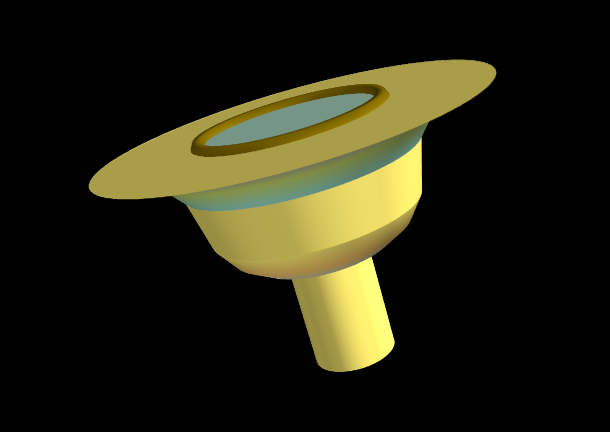
\includegraphics[scale=0.25]{slika3.png}
\label{slika3a}}\hspace*{0.5cm}
\subfigure[dio]{
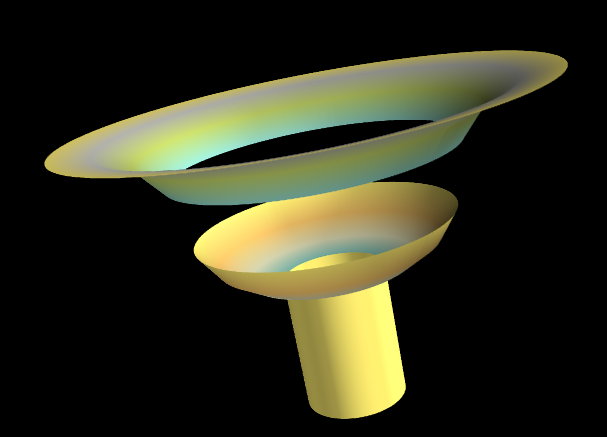
\includegraphics[scale=0.25]{slika3a.png}
\label{slika3b}}
\vspace*{-10pt}
\caption{}
\label{slika3}
\end{figure}
\noindent Dijelove prikazane na slici \ref{slika3b} modeliramo na sljede\'ci na\v{c}in. Jedan od tih dijelova modeliramo pomo\'cu cilindra
$$r(u,v)=\big(3\sin{u},\,3\cos{u},\,v\big),\quad u\in[0,2\pi],\ v\in[0,8].$$
Preostala dva dijela modeliramo pomo\'cu rotacijskih ploha tako da krivulje
\begin{gather*}
c_1(t)=(0,3+5\cos{t},13+5\sin{t}),\quad t\in\big[\tfrac{3}{2}\pi,\tfrac{15}{8}\pi\big]\\[5pt]
c_2(t)=(0,14+6\cos{t},13+5\sin{t}),\quad t\in\big[\tfrac{\pi}{2},\tfrac{7}{8}\pi\big]
\end{gather*}
zarotiramo oko $z$-osi. Nadalje, prazninu izme\dj u dijelova prikazanih na slici \ref{slika4a} popunimo na sljede\'ci na\v{c}in.
U $yz$-ravnini uzmemo du\v{z}inu koja spaja te dijelove kako je prikazano na slici \ref{slika4b} (\v{z}uta du\v{z}ina) i nakon
toga tu du\v{z}inu zarotiramo oko $z$-osi.%\par  
\begin{figure}[!h]
\centering
\subfigure[dio]{
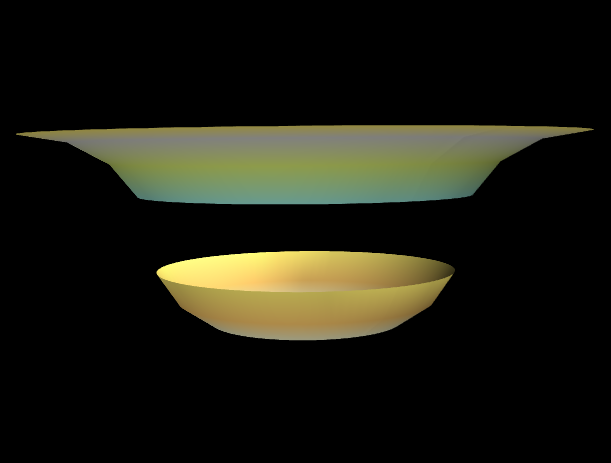
\includegraphics[scale=0.25]{slika4.png}
\label{slika4a}}\hspace*{0.5cm}
\subfigure[dio]{
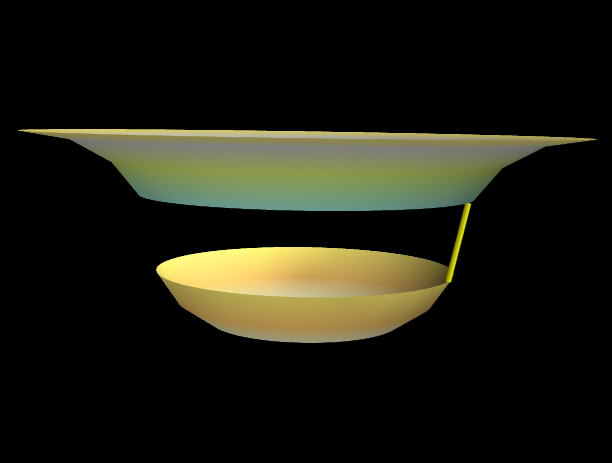
\includegraphics[scale=0.25]{slika4a.png}
\label{slika4b}}
\vspace*{-10pt}
\caption{}
\label{slika4}
\end{figure} 
\noindent Kona\v{c}no, dio prikazan na slici \ref{slika5} modeliramo preko sljede\'cih formula
\begin{alignat*}{3}
x&=6u_1\sin{v_1}&\qquad\quad x&=14u_2\sin{v_2}&\qquad\quad x&=6.5\cos{t}\\[3pt]
y&=6u_1\cos{v_1}& y&=14u_2\cos{v_2}& y&=6.5\sin{t}\\[3pt]
z&=18& z&=18& z&=18
\end{alignat*}
gdje je $u_1\in[0,1],\, v_1\in[0,2\pi],\, u_2\in[0.5,1],\, v_2\in[0,2\pi],\, t\in[0,2\pi]$.\par\vspace*{5pt}
\begin{figure}[!h]
\centering
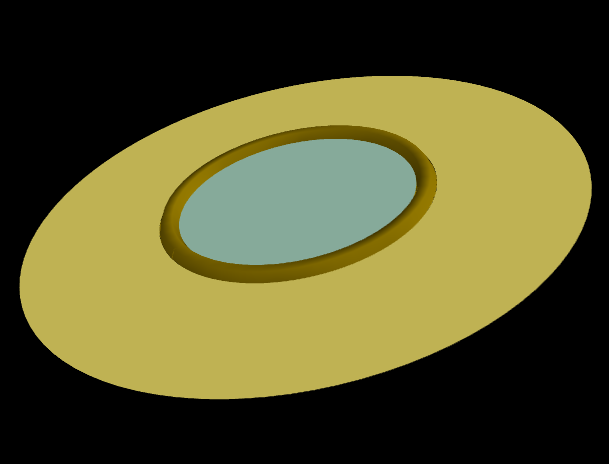
\includegraphics[scale=0.25]{slika5.png}
\vspace*{-10pt}
\caption{}
\label{slika5}
\end{figure}\vspace*{5pt}
\noindent Ako u ovom trenutku prika\v{z}emo istovremeno dijelove na slikama \ref{slika2} i \ref{slika3a}, dobit \'cemo
scenu kakva je prikazana na slici \ref{slika6a}. Translacijom za odgovarajući vektor ta dva dijela se mogu spojiti
kako je prikazano na slici \ref{slika6b}.\par\vspace*{5pt}
\begin{figure}[!h]
\centering
\subfigure[dio]{
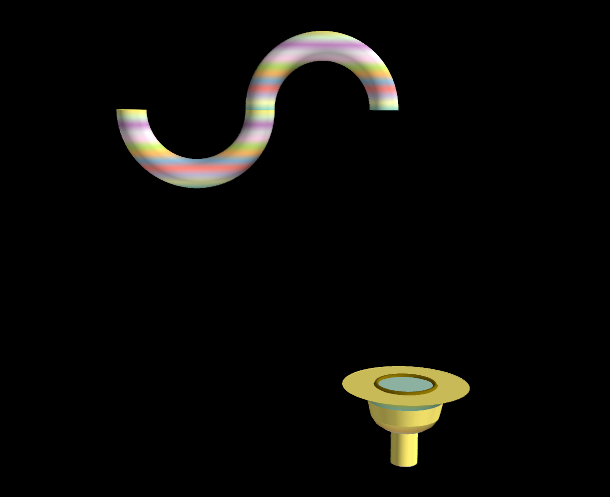
\includegraphics[scale=0.22]{slika6.png}
\label{slika6a}}\hspace*{0.5cm}
\subfigure[dio]{
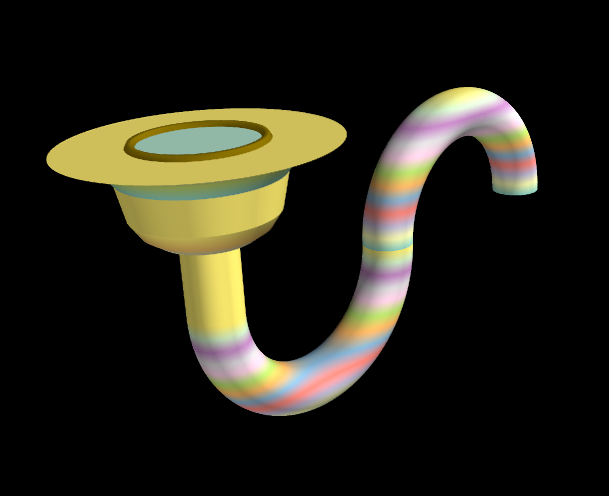
\includegraphics[scale=0.22]{slika6a.png}
\label{slika6b}}
\vspace*{-10pt}
\caption{}
\label{slika6}
\end{figure} 

\newpage
\noindent Modeliranje oblika prikazanog na slici \ref{slika7a} opisat \'cemo u nekoliko koraka.
\begin{figure}[t]
\centering
\subfigure[dio]{
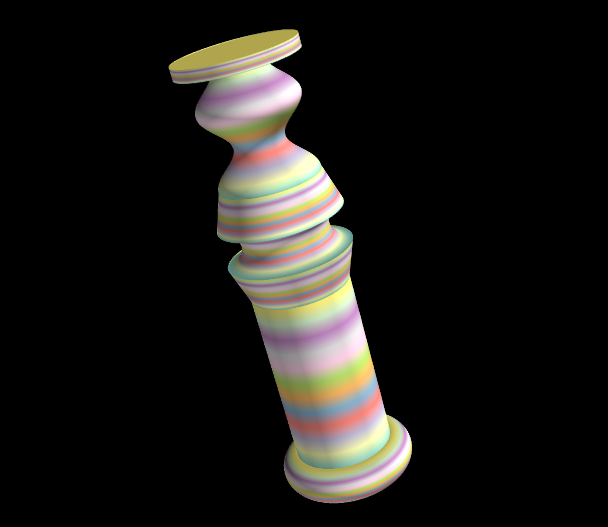
\includegraphics[scale=0.22]{slika7.png}
\label{slika7a}}\hspace*{0.5cm}
\subfigure[dio]{
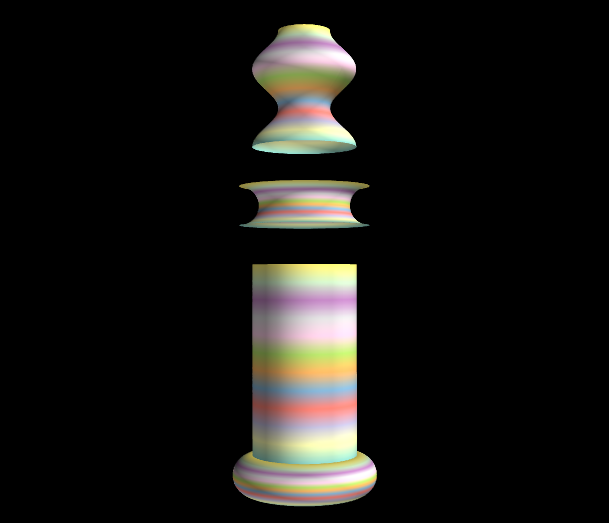
\includegraphics[scale=0.22]{slika7a.png}
\label{slika7b}}
\vspace*{-10pt}
\caption{}
\label{slika7}
\end{figure}
Dijelove prikazane na slici \ref{slika7b} modeliramo tako da krivulje
\begin{align*}
c_1(t)&=(0,8+3\cos{t},8+3\sin{t}),\quad t\in\big[\tfrac{-\pi}{2},\tfrac{\pi}{2}\big]\\[5pt]
c_2(t)&=(0,10+3\cos{t},49+3\sin{t}),\quad t\in\big[\tfrac{\pi}{2},\tfrac{3}{2}\pi\big]\\[5pt]
c_3(t)&=\big(0,6+2\cos{t},\tfrac{6}{\pi}t+58\big),\quad t\in[0,3\pi]\\[5pt]
c_4(t)&=(0,8,11+29t),\quad t\in[0,1]
\end{align*}
\begin{figure}[!h]
\centering
\parbox{5cm}{
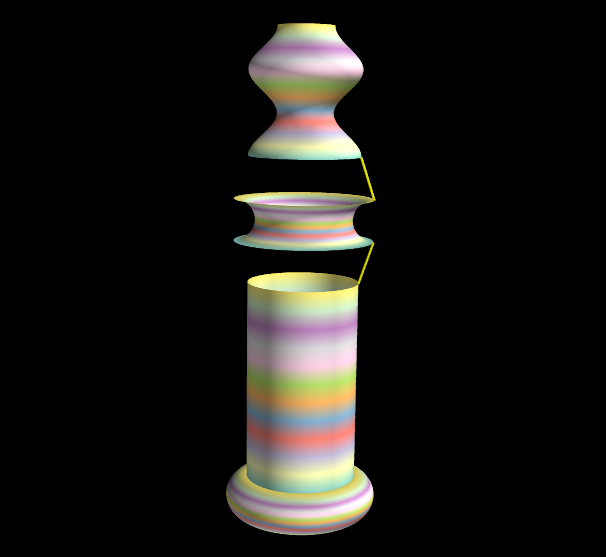
\includegraphics[scale=0.23]{slika7b.png}
\caption{}
\label{slika7c}}
\qquad
\begin{minipage}{5cm}
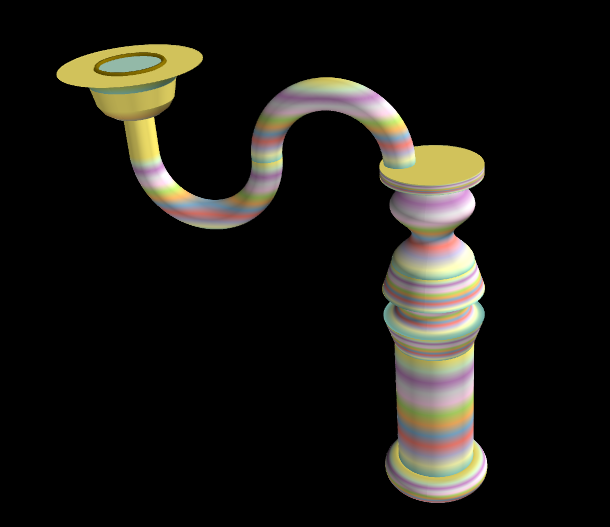
\includegraphics[scale=0.23]{slika8.png}
\caption{}
\label{slika8}
\end{minipage}
\end{figure}
zarotiramo oko $z$-osi. Praznine izme\dj u dijelova prikazanih na slici \ref{slika7b} popunimo tako da
u $yz$-ravnini uzmemo du\v{z}ine koje spajaju odgovaraju\'ce dijelove kako je prikazano na slici \ref{slika7c} (\v{z}ute du\v{z}ine) i nakon toga te du\v{z}ine zarotiramo oko $z$-osi. Sve preostale dijelove modela sa slike \ref{slika7a} modeliramo pomo\'cu ploha
\begin{alignat*}{4}
x&=u\sin{v}&\qquad\quad x&=1.2u\sin{v}&\qquad\quad x&=1.2u\sin{v}&\qquad\quad x&=9.6\sin{v}\\[3pt]
y&=u\cos{v}&\qquad\quad y&=1.2u\cos{v}&\qquad\quad y&=1.2u\cos{v}&\qquad\quad y&=9.6\cos{v}\\[3pt]
z&=5&\qquad\quad z&=76&\qquad\quad z&=78&\qquad\quad z&=76+0.25u 
\end{alignat*}
gdje je $u\in[0,8],\,v\in[0,2\pi]$.\\[5pt]
Ako prika\v{z}emo istovremeno modele na slikama \ref{slika6b} i \ref{slika7a}, dobit \'cemo model prikazan na slici \ref{slika8}. 
Odgovaraju\'cim rotacijama oko $z$-osi modela sa slike \ref{slika6b} kona\v{c}no dobijemo model svije\'cnjaka koji je prikazan na slici \ref{slika1}.      

 
\end{document}
